\documentclass[a4paper, 12pt]{article}
\usepackage[utf8]{inputenc}
\usepackage[ngerman]{babel}
\usepackage{amsmath}
\usepackage{booktabs}
\usepackage{graphicx}

\title{Bloom Filter}
\author{Jan Werren, Xeno Suter}
\date{Dezember 2024}
\begin{document}

\maketitle
\tableofcontents

\newpage

\section{Was ist ein Bloom Filter und die Idee dahinter}\label{sec:was-ist-ein-bloom-filter-und-die-idee-dahinter}
Ein Bloom-Filter ist eine probabilistische Datenstruktur, die überprüft, ob ein Element in einem Set enthalten ist.
Er basiert auf einem BitSet und mehreren Hash-Funktionen (murmur3-128). 
Neue Elemente werden durch Setzen von Bits im Array hinzugefügt.
Um zu testen, ob ein Element enthalten ist, wird überprüft, ob alle relevanten Bits der Hashes auf \texttt{1} gesetzt sind.

\section{Vor- und Nachteile von Bloom Filtern}\label{sec:vor--und-nachteile-von-bloom-filtern}

\subsection{Vorteile}\label{subsec:vorteile}
\begin{itemize}
    \item Sehr speichereffizient im Vergleich zu traditionellen Datenstrukturen wie Sets.
    Speicherplatzkomplexität: $O(m)$ (wobei $m$ die Anzahl der Bits im Bloom-Filter ist).
    \item Schnelle Einfüge- und Prüfoperationen (Zeitkomplexität: $O(k)$, wobei $k$ die Anzahl der Hash-Funktionen ist).
    \item Keine \textit{false negatives} möglich.
    Ein Element, das nicht im Set ist, wird immer korrekt als nicht enthalten erkannt.
\end{itemize}

\subsection{Nachteile}\label{subsec:nachteile}
\begin{itemize}
    \item \textit{False positives} möglich.
    Ein Element, das nicht im Set ist, kann fälschlicherweise als enthalten erkannt werden.
    Die Wahrscheinlichkeit für ein \textit{false positive} steigt mit der Anzahl der Elemente im Set und der Anzahl der Hash-Funktionen.
    \item Keine Möglichkeit, die Anzahl der Elemente im Set zu bestimmen.
    \item Keine Entfernung von Elementen möglich (ausser mit \textit{Counting Bloom Filters}).
\end{itemize}

\section{Implementierung Bloom Filters}\label{sec:implementierung-bloom-filters}
\subsection{Struktur}\label{subsec:struktur}
Ein Bloom-Filter besteht aus einem Bit-Array der Grösse $m$ und $k$ Hash-Funktionen.
Die Hash-Funktionen werden verwendet, um die Positionen im Bit-Array zu berechnen, an denen die Bits gesetzt werden.
Die Anzahl der Hash-Funktionen beeinflusst die Wahrscheinlichkeit von \textit{false positives}.

\section{Fehlerwahrscheinlichkeit}
Die Fehlerwahrscheinlichkeit wurde wie folgt getestet:
\begin{itemize}
    \item Eine definierte Anzahl von Wörtern aus einer Datei \texttt{words.txt} wurde in den Bloom-Filter eingefügt.
    \item Anschliessend wurden 100'000 zufällige Wörter generiert, die sicher nicht in \texttt{words.txt} enthalten waren.
    \item Für jedes zufällige Wort wurde überprüft, ob der Bloom-Filter es als enthalten markiert.
    \item Die experimentelle Fehlerwahrscheinlichkeit wurde als Verhältnis der \textit{false positives} zur Anzahl der getesteten Wörter berechnet.
    \item Des Weiteren wurde die theoretische Fehlerwahrscheinlichkeit berechnet. Mit folgender Formel:
    \[
        P_{\text{false}}(m, n) = \left( 1 - \left( 1 - \frac{1}{m} \right)^{k \cdot n} \right)^k
    \]
    wobei
    \[
        k = \left\lceil \frac{m}{n} \ln(2) \right\rceil
    \]
\end{itemize}

\subsection{Ergebnisse der Fehlerwahrscheinlichkeit}\label{subsec:ergebnisse-der-fehlerwahrscheinlichkeit}
Die berechnete Fehlerwahrscheinlichkeit stimmt eng mit der theoretischen Wahrscheinlichkeit überein
Für $n = 1000$ Elemente und $p = 0.01$ ergab der Test:
\begin{itemize}
    \item Berechnete Fehlerwahrscheinlichkeit: $0.01$
    \item Experimentelle Fehlerwahrscheinlichkeit: $0.0101$
\end{itemize}

\section{Beispiel aus der Praxis}\label{sec:beispiel-aus-der-praxis}
Ein typisches Anwendungsbeispiel für Bloom-Filter ist in verteilten Systemen wie \textbf{Apache Cassandra}.
Cassandra verwendet Bloom-Filter, um schnell zu überprüfen, ob ein bestimmter Schlüssel in einer Datenbank vorhanden sein könnte, bevor eine ressourcenintensive Abfrage durchgeführt wird.
Dadurch wird die Abfragezeit erheblich reduziert.

\section{Programmausgabe}\label{sec:programmausgabe}
\begin{figure}[h!]
    \centering
    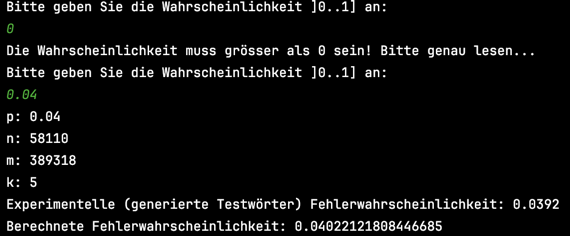
\includegraphics[width=\textwidth]{example_output}
    \caption{Screenshot der Programmausgabe}
    \label{fig:output}
\end{figure}

\end{document}